\documentclass[tikz,border=8pt]{standalone}
% Shared look for every TikZ diagram. Load with \input{../../tools/tikz-style.tex}
\usepackage[T1]{fontenc}
\usepackage{lmodern}
\renewcommand{\sfdefault}{lmr}  % diagrams use the same serif as the text
\usetikzlibrary{arrows.meta, positioning, shapes.geometric, calc, fit, backgrounds}
\definecolor{cblue}{HTML}{4C78A8}
\definecolor{corange}{HTML}{F58518}
\definecolor{cgreen}{HTML}{54A24B}
\definecolor{cred}{HTML}{E45756}
\definecolor{cpurple}{HTML}{B279A2}
\definecolor{cgrey}{HTML}{6B6B6B}
\tikzset{
  every picture/.style={font=\sffamily, line width=1.2pt},
  box/.style={draw=#1, fill=#1!12, rounded corners=4pt, align=center, inner sep=7pt, minimum height=1.1cm},
  box/.default=cgrey,
  arrow/.style={-{Stealth[length=3mm]}, draw=cgrey, line width=1.4pt},
  title/.style={font=\sffamily\bfseries\Large},
  note/.style={font=\sffamily\small, text=cgrey, align=center},
}
\AtBeginDocument{\hyphenpenalty=10000 \exhyphenpenalty=10000}

\begin{document}
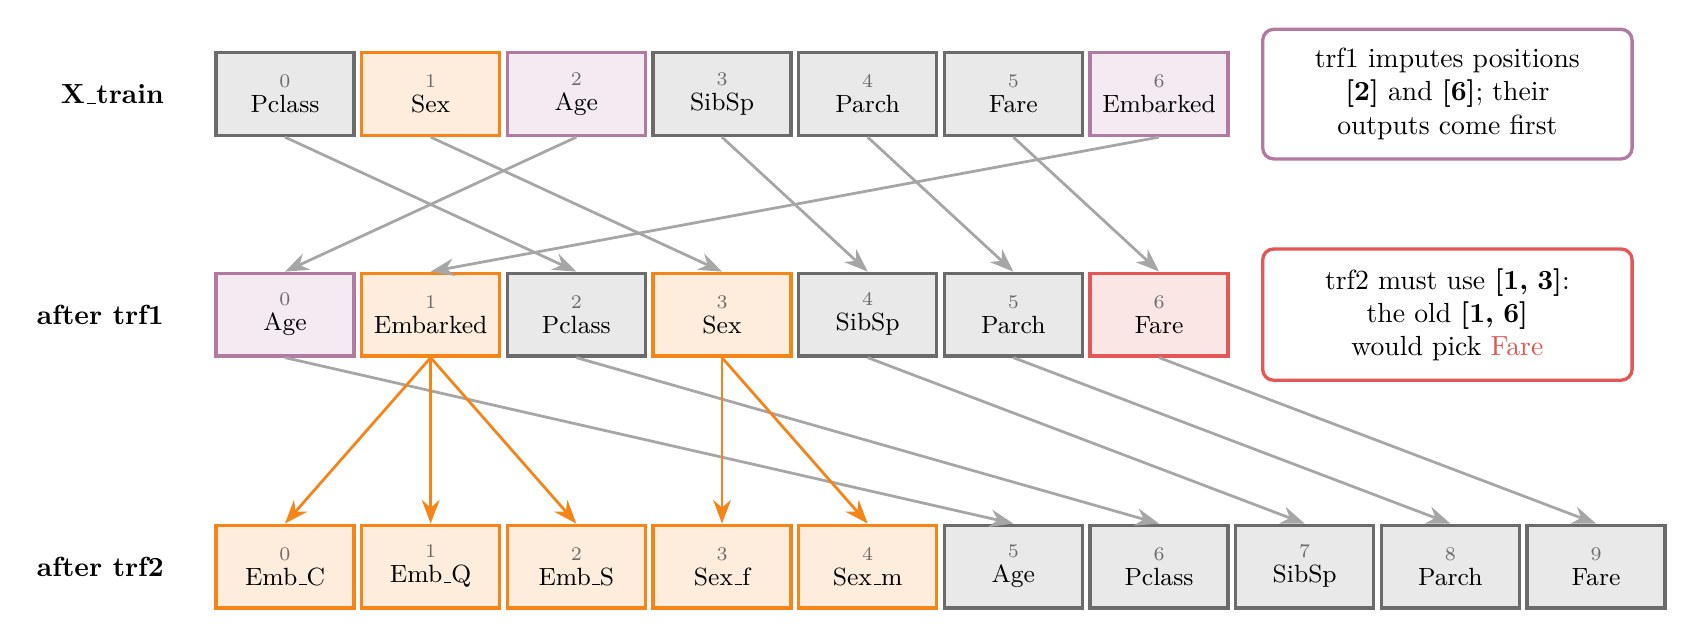
\begin{tikzpicture}[cell/.style={draw=#1, fill=#1!15, minimum width=1.75cm, minimum height=1.05cm, align=center, inner sep=2pt, font=\sffamily\small}]
  \def\w{1.85}
  \newcommand{\cl}[2]{{\scriptsize\color{cgrey}#1}\\[-2pt]#2}
  % row A: the input columns
  \node[font=\sffamily\bfseries, anchor=east] at (-1.4,0) {X\_train};
  \foreach \n/\c [count=\i from 0] in {Pclass/cgrey, Sex/corange, Age/cpurple, SibSp/cgrey, Parch/cgrey, Fare/cgrey, Embarked/cpurple} {
    \node[cell=\c] (a\n) at (\w*\i,0) {\cl{\i}{\n}};
  }
  % row B: after trf1, the imputed columns come first
  \node[font=\sffamily\bfseries, anchor=east] at (-1.4,-2.8) {after trf1};
  \foreach \n/\c [count=\i from 0] in {Age/cpurple, Embarked/corange, Pclass/cgrey, Sex/corange, SibSp/cgrey, Parch/cgrey, Fare/cred} {
    \node[cell=\c] (b\n) at (\w*\i,-2.8) {\cl{\i}{\n}};
  }
  \foreach \n in {Pclass, Sex, Age, SibSp, Parch, Fare, Embarked} { \draw[arrow, cgrey!60, line width=1pt] (a\n.south) -- (b\n.north); }
  % row C: after trf2, the one-hot columns come first
  \node[font=\sffamily\bfseries, anchor=east] at (-1.4,-6) {after trf2};
  \foreach \n/\l/\c [count=\i from 0] in {eC/Emb\_C/corange, eQ/Emb\_Q/corange, eS/Emb\_S/corange, sF/Sex\_f/corange, sM/Sex\_m/corange,
                                         Age/Age/cgrey, Pclass/Pclass/cgrey, SibSp/SibSp/cgrey, Parch/Parch/cgrey, Fare/Fare/cgrey} {
    \node[cell=\c] (c\n) at (\w*\i,-6) {\cl{\i}{\l}};
  }
  \foreach \n in {Age, Pclass, SibSp, Parch, Fare} { \draw[arrow, cgrey!60, line width=1pt] (b\n.south) -- (c\n.north); }
  \foreach \t in {eC, eQ, eS} { \draw[arrow, corange, line width=1pt] (bEmbarked.south) -- (c\t.north); }
  \foreach \t in {sF, sM} { \draw[arrow, corange, line width=1pt] (bSex.south) -- (c\t.north); }
  % call-outs
  \node[box=cpurple, fill=white, text width=4.2cm, anchor=west] at (\w*6.7,0) {trf1 imputes positions \textbf{[2]} and \textbf{[6]}; their outputs come first};
  \node[box=cred, fill=white, text width=4.2cm, anchor=west] at (\w*6.7,-2.8) {trf2 must use \textbf{[1, 3]}:\\the old \textbf{[1, 6]} would pick \textcolor{cred}{Fare}};
\end{tikzpicture}
\end{document}
